% 
\newglossaryentry{X}
{
  type=differential-privacy,
  name={$\ensuremath{X} $},
  description={Set of locations for a user. ($R^2$)},
}
\newglossaryentry{Z}
{
  type=differential-privacy,
  name={$\ensuremath{Z} $},
  description={For every $x \in X$ a perturbed location $z \in Z$ is reported.},
}
\newglossaryentry{K}
{
  type=differential-privacy,
  name={$K(x)(Z)$},
  description={Randomization method for $x \in X$ and output $z \in Z$.},
}
\newglossaryentry{Epsilon}
{
  type=differential-privacy,
  name={$\ensuremath{\epsilon} $},
  description={The privacy budget $\epsilon$ determines the amount of noise that is added.
    },
}
\newglossaryentry{Pr}{
  type=differential-privacy,
  name={$Pr(K(x_i) \in (Z))$},
  description={Probability of reporting $x \in X$ for $z \in Z$}
}


\section{Differential privacy} \label{section:dp}
In practice, data is often sent to a central storage point.
This requires trust, and because all data is collected in one place, the risk of private data leakage becomes very high.
By applying \gls{dp}, noise can be added to the data to protect it.
This principle is illustrated in the following figure:
\begin{figure}[H]
  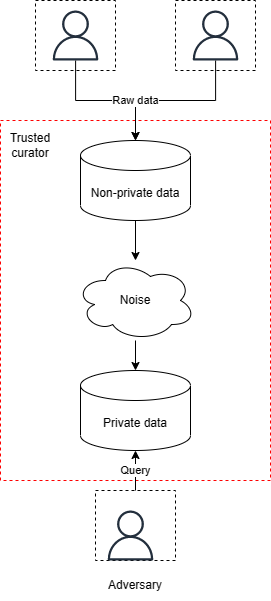
\includegraphics[width=1\textwidth]{TheorethicalFramework/Differential privacy/central-dp.png}
  \caption{General approach for setting up (central) differential privacy.}
  \label{fig:central-dp}
\end{figure}

\begin{enumerate}
  \item The system that receives data from users. It is assumed in this setting that the system is trustworthy and that the data is securely stored.
  \item The data is collected and stored in a database, and the noise is added by a differential privacy mechanism.
  \item Someone interested in the data, such as a data scientist, can access and analyze the private data.
\end{enumerate}
To a certain extent, a user's privacy would be ensured with differential privacy. \newline

Although differential privacy solves privacy problems, it remains challenging to calibrate the mechanism.
There is an important trade-off between utility and privacy for the adversary.
For example, a data scientist wants accurate data. At the same time, the noise must be sufficient to prevent an attacker from obtaining too much information.

For this reason, a few sections will be devoted to outlining the mathematical background of differential privacy.
We will examine which factors influence this calibration and whether other methods contribute.
Afterward, we will further explain other types of differential privacy (local and geo-indistinguishable) similarly.

%\glsaddall
%\leading{10pt}
%\printglossary[type=differential-privacy, nonumberlist]
%\begin{figure}[h]
%  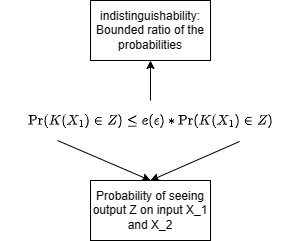
\includegraphics{TheorethicalFramework/Differential privacy/master-thesis-Differential privacy illustration.png}
%  \caption{Randomization function $K$ gives $\epsilon$-differential privacy for all elements in $D_1$ and $D_2$ if they differ at most one element. \citep{dwork_differential_2006}}
%  \label{fig:definition-dp}
%\end{figure}

\newpage
\subsection{Definitions}
We examine the different notations and types of differential privacy we consider in this research.

\subsubsection{$\epsilon$-differential privacy}
Dwork et al. formulated the notion of privacy: Participating in a database should not significantly increase the risk of an individual's privacy being compromised \cite{dwork_differential_2006}.
This is mathematically formulated in the same research named \gls{dp}.
Using the definition of privacy, it is formulated as the maximal possible change when adding or removing a single record \citep{dwork_differential_2006, friedman_data_2010}.
This is reflected using the formal mathematical formulation as formulated by Dwork et al:
\begin{equation}
  {\mathrm{Pr}}[K(D_{1})\in S]\leq\exp(\epsilon) \cdot {\mathrm{Pr}}[K(D_{2})\in S]
  \label{pure-dp}
\end{equation}
So, given a randomization function $K$, it gives $\epsilon$-differential privacy if dataset $D_1$ and $D_2$ are differing at most one element \citep{dwork_differential_2006}.
The $\epsilon$ determines the amount of noise (privacy budget) \citep{friedman_data_2010}.
The lower the value of $\epsilon$, the higher the privacy guarantee.
In this regard, it is essential for a method that ensures differential privacy to consider this.
For this reason, a common way to calibrate the $\epsilon$ is to calculate the sensitivity.
This value is calculated based on the impact of a function or query on the data.
For example, if there is a method called $sum$ for the summation of data points, the method's sensitivity is 1.
This is because removing one data point would significantly affect the outcome, and $\epsilon$-differential privacy could no longer be guaranteed.
It is also mathematically defined by Dwork et al.:
\begin{equation}
  \Delta f=\operatorname*{max}_{D_{1},D_{2}}\|f(D_{1})-f(D_{2})\|_{1}
  \label{sensitivity-dp}
\end{equation}
\subsubsection{$(\epsilon, \delta)$-differential privacy}
The formal notion of differential privacy has only the privacy budget $\epsilon$ as a parameter.
This formulation is strict, but most methods relax this a little, with $(\epsilon, \delta)$:
\begin{equation}
  {\mathrm{Pr}}[K(D_{1})\in S]\leq e^{\epsilon} \cdot {\mathrm{Pr}}[K(D_{2})\in S] + \delta
  \label{approxiate-dp}
\end{equation}
This equation means the sensitivity ($\delta$) loosens the formal definition of differential privacy.
The $\delta$ is added to the upper bound of the exponential, so the desired noise can be higher.
%The purpose of $\epsilon$ now is to calibrate the desired amount of privacy.
To some extent, the delta represents the probability of the algorithm leaking information \citep{aitsam_differential_2021}.
With $\epsilon$-differential privacy, there would be no difference in the case of information leakage ($\delta$ = 0).
However, with $(\epsilon, \delta)$-differential privacy, the information can leak up to the probability of delta.
\newpage
\subsubsection{$\epsilon$-local differential privacy}
As the name suggests, \gls{ldp} is executed on the client side instead of on the server (See Figure \ref{fig:central-dp}).
%The principle of \gls{ldp} is illustrated in figure \ref{fig:local-dp}.
Local differential privacy removes the "trusted" curator/ server, preventing sensitive data leakage even if an attacker gains access to the dataset \citep{del_rey_comprehensive_2020}.
The principle of \gls{ldp} is illustrated in the following figure:
\begin{figure}[H]
  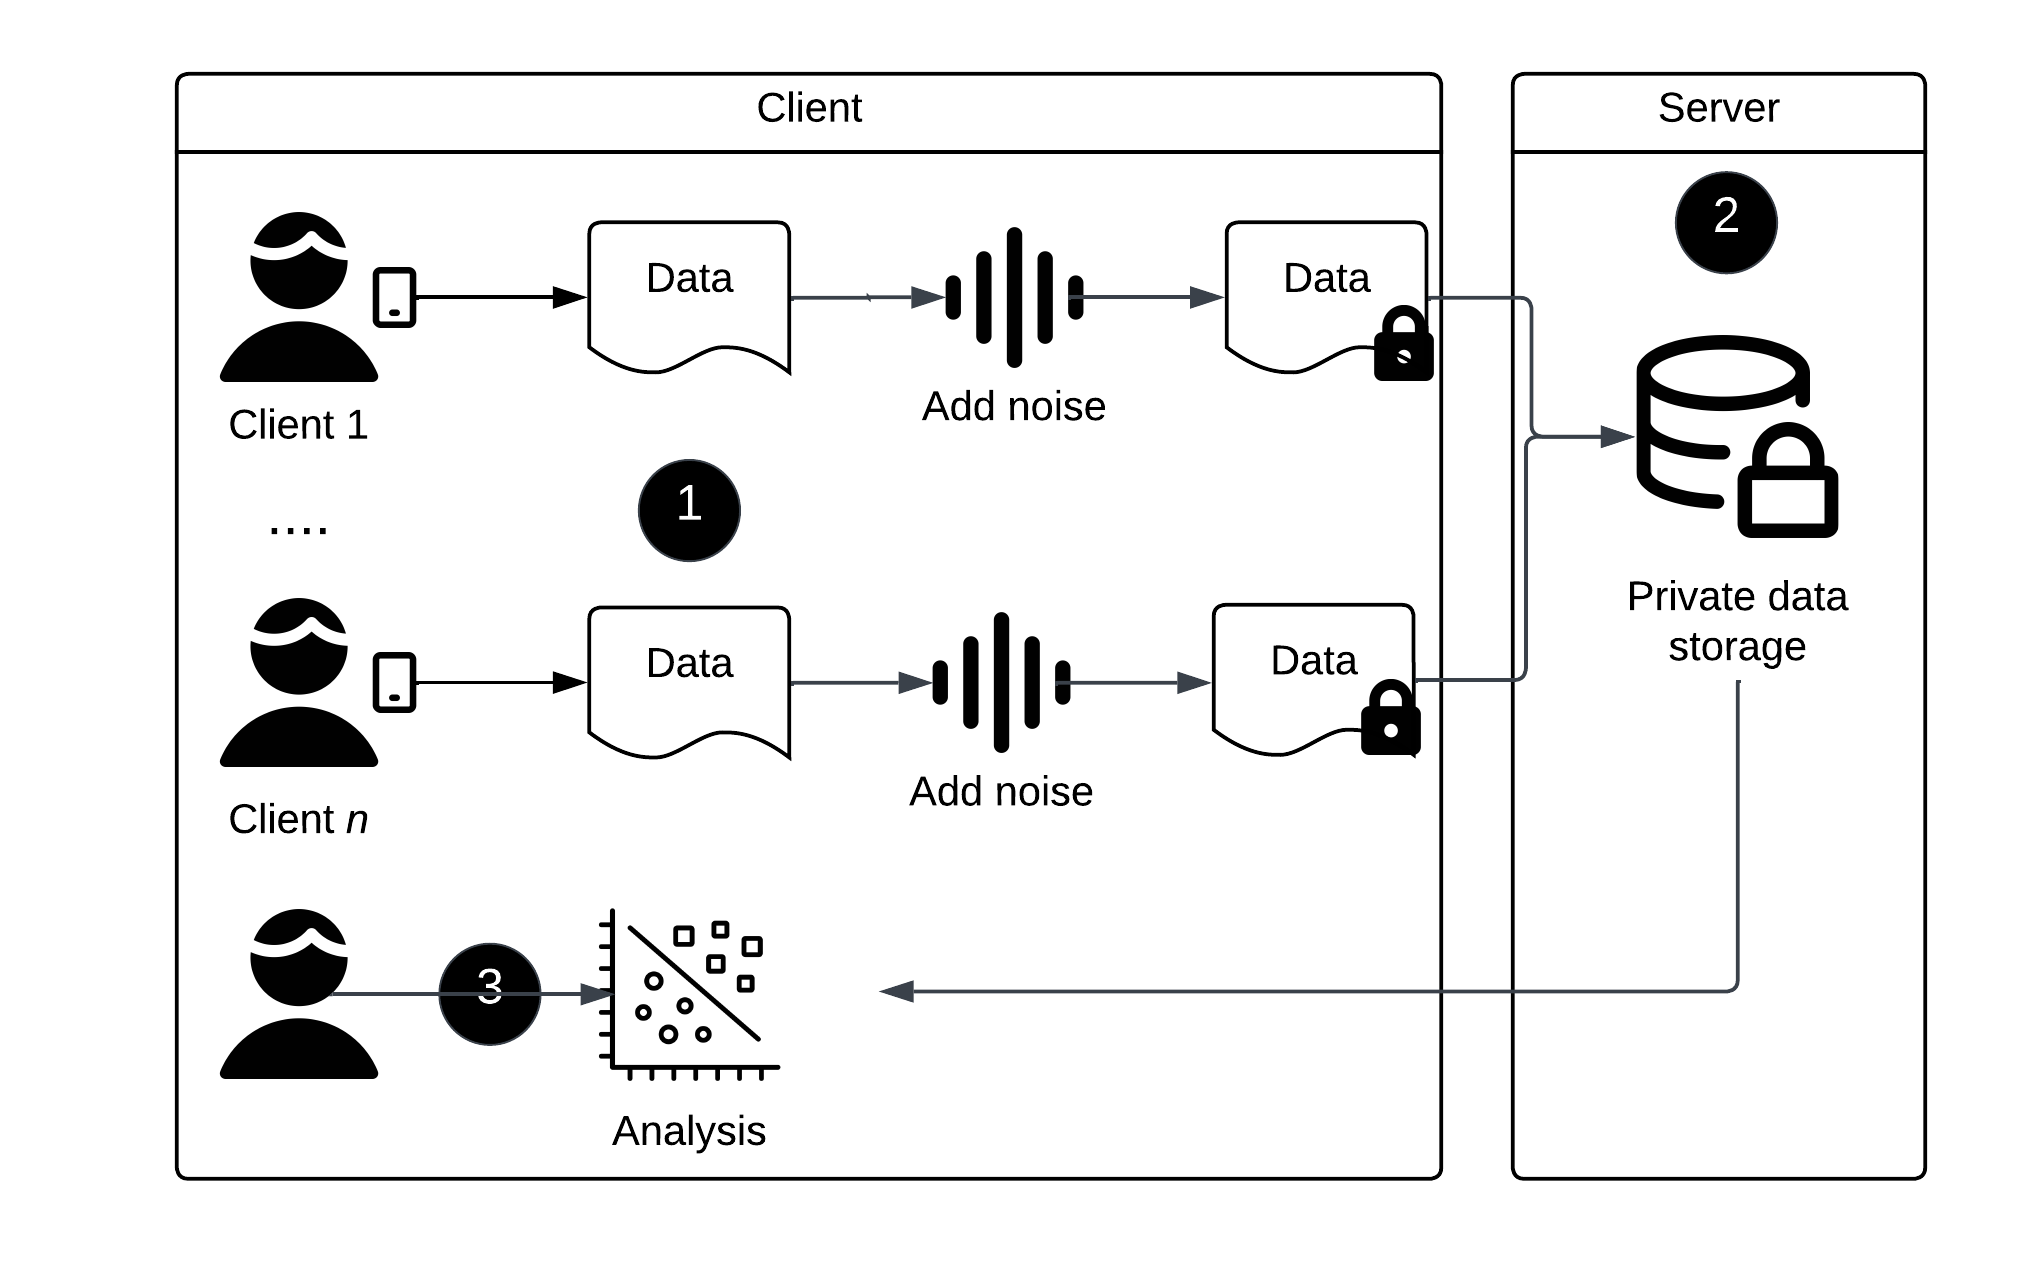
\includegraphics[width=1\textwidth]{TheorethicalFramework/Differential privacy/local-dp.png}
  \caption{Local differential privacy, which moves the noise-adding step to the client side.}
  \label{fig:local-dp}
\end{figure}
\begin{enumerate}
  \item The clients have their data record(s) locally (client-sided) and add noise to them directly. This way, the server never receives plain data.
  \item The data is sent to the server and can just be stored securely.
  \item As with \gls{dp}, a stakeholder interested in the data receives it and can analyze it.
\end{enumerate}
%The definition for \gls{ldp} is the as for equation \ref{approxiate-dp} with $\delta = 0$ being equal to equation \ref{pure-dp}.
Local differential privacy has two different frameworks.
It can be set up as interactive or non-interactive \citep{del_rey_comprehensive_2020}.
\newline
Where interactive can be distinguished as either sequentially interactive or fully interactive \footnote{Image source: \url{https://www.majos.net/focs_19_talk.pdf}}:
\begin{figure}[H]
  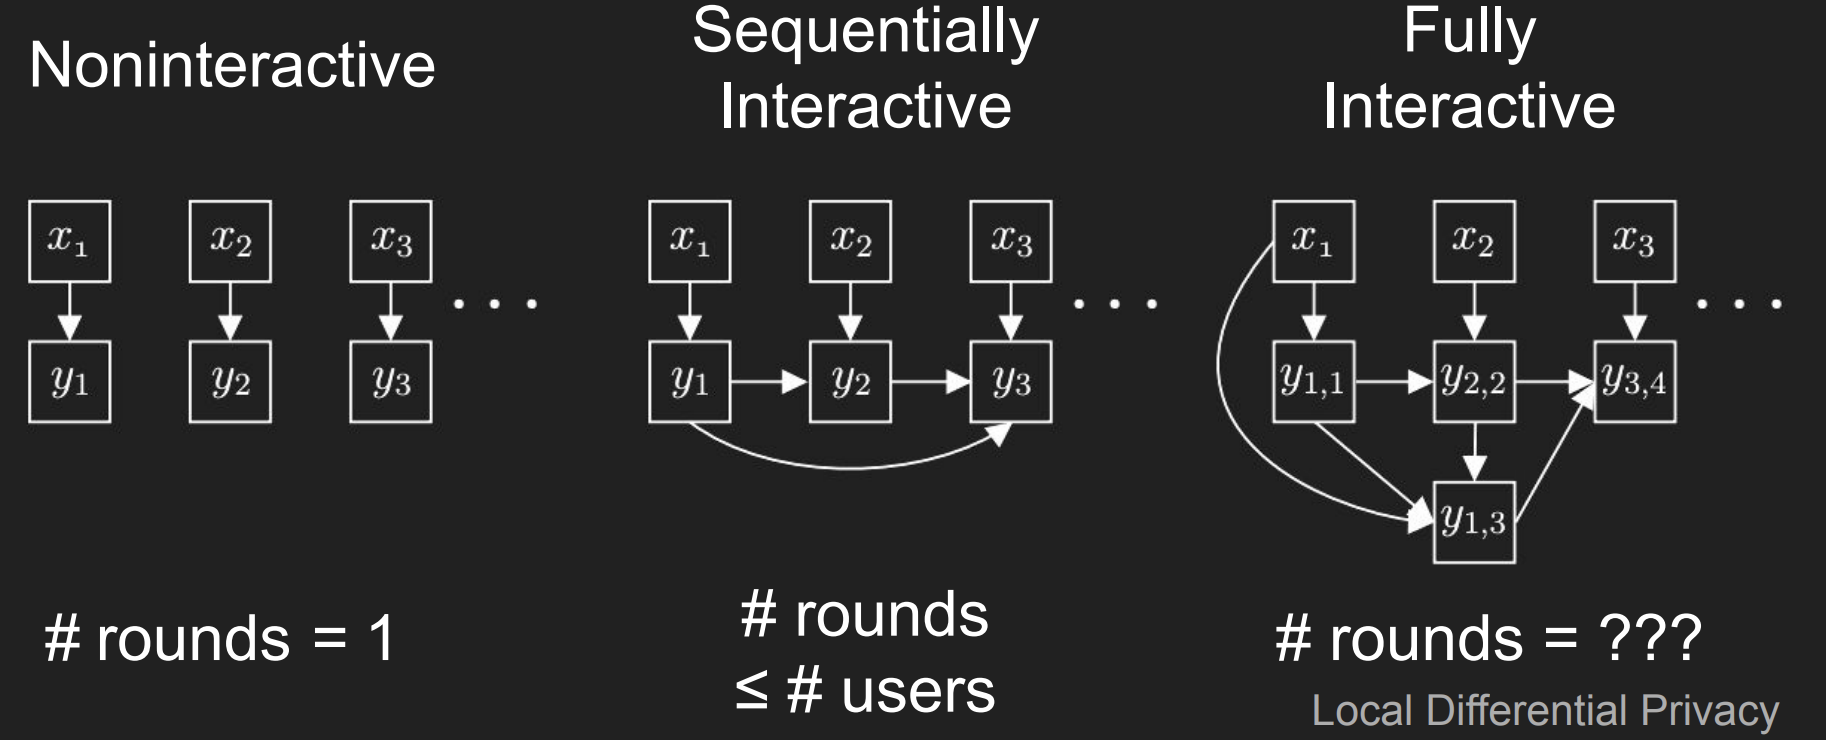
\includegraphics[width=\textwidth]{TheorethicalFramework/nont-interactive-versus-interactive.png}
  \caption{Non-interactive versus sequentially interactive versus fully interactive local differential privacy \citep{joseph_role_2019-1}}
  \label{fig:non-interactive-versus-interactive}
\end{figure}
In the non-interactive framework, the privacy mechanism operates on a single data instance (e.g., users’ smartphones) without requiring interaction with other clients or between data points.
This interaction means that each data point is perturbed independently, and the privacy guarantees are achieved without communication or coordination between the data points.
In the interactive framework, the privacy mechanism involves a process of iterative interactions between users and clients.
Each data point considers other data points' responses to determine its own perturbation or privacy level.
The interactions can occur through a communication channel, where data points exchange information with each other or a trusted mediator.
The iterative nature of the interactive framework allows for refining and improving the privacy guarantees based on the global knowledge of the data set.

In figure \ref{fig:non-interactive-versus-interactive}, the different interactive types are visualized, where the most notable difference is the around of rounds \citep{xiongComprehensiveSurveyLocal2020}.
A sequentially interactive framework passes at most one message between data points.
A fully interactive framework could provide an unknown and unlimited amount of messages between data points.
The interactive framework has unlimited access to other data points, which is most suitable for practical appliances \citep{xiongComprehensiveSurveyLocal2020}.
The practical applications are better because the data points' mutual correlation also contributes to utility \citep{wang_comprehensive_2020}.

\subsubsection{$\epsilon$-geo-indistinguishability} \label{theory:geo-indistinguishability}
The last and most important type of differential privacy for this study is \gls{gi}.
%This is a type of differential privacy that is specifically designed for location data.
\gls{gi} can be applied to preserve privacy using a differential privacy method specific to spatial data \citep{DBLP:journals/corr/abs-1212-1984}.
Consider a local-based system (LBS) that provides a map service to its users (e.g., Google Maps).
The users can query the LBS for a route from their current location to a destination.
%This information is private, and the LBS should not be able to track the user's location.
Instead of the exact (private) location, the LBS should only receive an approximate location enough to provide the service at an adequate level.
This approximation happens entirely locally, so no central server exists. \newline
In addition to this, the mechanism provides an initiative way of calibrating the desired privacy, which is illustrated in the following figure:
\begin{figure}[H]
\centering
  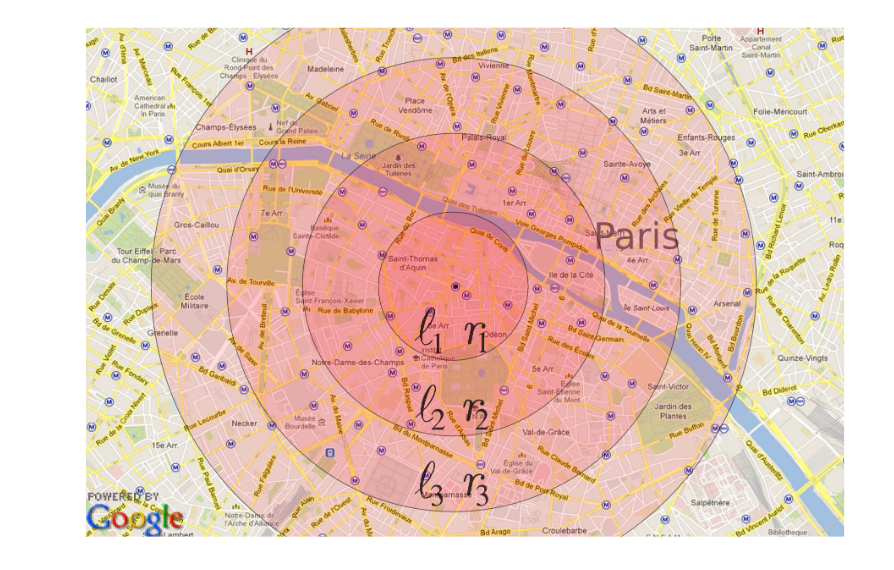
\includegraphics[width=0.5\textwidth]{TheorethicalFramework/geo-indistinguishability.png}
  \caption{Visualisation of radius $r$ with $l$ to provide Geo-indistinguishability mechanism \citep{DBLP:journals/corr/abs-1212-1984}}
  \label{fig:geo-indistinguishability}
\end{figure}
The figure shows two variables to configure the amount of noise: $r$ and $l$.
Users provide a privacy radius $r$, and the noise is added and preserved within this radius.
A fake location $z$ is generated within this radius based on the Euclidean distance $d$.
The amount of noise can be configured using the privacy level $l$.
Thus, a higher $r$ or/and $l$ provides a higher privacy guarantee. \newline
In a practical scenario, the $r$ and $l$ variables are combined to obtain the privacy budget $\epsilon$.
The privacy budget is obtained by using the formula $\epsilon = \frac{l}{r}$, and the $\epsilon$ is used as input for the \gls{gi} mechanism to calibrate the noise. \newline
The formal definition of \gls{gi} is the following \citep{DBLP:journals/corr/abs-1212-1984}:
\begin{equation}
  K(x)(Z) \le e^{\epsilon \cdot d(x,x')} K(x')(Z) \ for \ all \ x,x' \in X, Z \subseteq X 
  \label{algo:2d-geo-indistinguishability}
\end{equation}
According to the Andres et al., the mechanism provides ($\epsilon$)-geo-indistinguishability for any $z \in Z$ that is generated within the radius $r$ \citep{DBLP:journals/corr/abs-1212-1984}.
%An extension of this is called $d_x$-privacy, a more general notation of distance-aware differential privacy.
%Therefore, the definition for \gls{gi} is $d_2$-privacy, but it is essentially the same as the proof provided for \gls{gi}.
\subsection{Laplace mechanism} \label{theory:laplace}
The previous sections have explained the different privacy frameworks that exist for differential privacy.
In the current section, we explain an important (L)DP mechanism on which the mechanism of \gls{gi} is based.
We provide the definition, laying the groundwork for the mechanisms of \gls{gi}.

The Laplace mechanism, initially proposed in the same paper as a foundational concept for differential privacy \citep{dwork_differential_2006},
introduces noise to the data based on a privacy budget ($\epsilon$).
Additionally, it incorporates a sensitivity parameter ($\delta$).
While the privacy budget determines the amount of noise to be added, sensitivity is used to calibrate the output based on the input \citep{del_rey_comprehensive_2020}.

The definition of the Laplace mechanism is as follows \citep{del_rey_comprehensive_2020}:
\begin{equation}
  M\left(f\left(x\right),\varepsilon\right)=f\left(x\right)+\left(Z_{1},\ldots,Z_{d}\right)
\end{equation}
Here, $Z$ is an independent collection of random variables drawn from the Laplace distribution.
The distribution scale is determined by the sensitivity of the function $f$ and the privacy budget $\epsilon$ \citep{del_rey_comprehensive_2020}.
Hence, the definition of the Laplace distribution is $Lap(\delta f/\epsilon)$, where $\delta f$ is the sensitivity of the function $f$. \newline

The sensitivity of $f$ can be calculated globally and locally.
Global sensitivity is independently calculated over two different datasets and is part of the original definition of \gls{dp} \citep{dwork_differential_2006}.
Usually, this is not the desired situation since local sensitivity always has more context of the dataset in question \citep{nissim_smooth_2007}.
As a result, the trade-off for noise is much more precise, and the balance between utility and privacy is much better.
The definition of sensitivity is the following \citep{nissim_smooth_2007}.
\begin{equation}
  LS(f,x)=\operatorname*{max}_{x^{\prime}\cdot d(x,x^{\prime})\leq1}|f(x)-f(x^{\prime})|
  \label{local-sensitivity}
\end{equation}
Here, $d$ is the distance between two datasets $x$ and $x'$.
The equation calculates the maximum difference between the output of $f(x)$ and $f(x')$, which should be at most $LS(f)$.
Because the sensitivity is the maximum difference between output and input, it looks a lot like the definition of \gls{dp} (Equation \ref{sensitivity-dp}).

In a practical scenario, it can be hard to calculate the local sensitivity.
To this end, the smooth sensitivity method was introduced by Nissim et al.  \citep{nissim_smooth_2007}.
This method aims at smoothing out the local sensitivity by focusing on reducing the noise without the risk of revealing more information.
Because it calculates many different configurations, a disadvantage of this method is that it can be computationally expensive.
Also, the introduction of this method makes Laplace preserve $(\epsilon, \delta)$-\gls{dp} instead of pure $\epsilon$-\gls{dp}.

%\subsubsection{Gaussian mechanism} \label{gaussian}
%Another mechanism that works comparably is the Gaussian mechanism.
%This mechanism makes use of the Gaussian distribution to add noise to the data.
%\todo[inline]{Explain more about Gaussian mechanism}
% This means, that if the sensitivity is low, the noise is as well.
% The metric is combined with the privacy budget $\epsilon$ to control the noise that is being added by a mechanism like Laplace \citep{friedman_data_2010}.


%The above attacks mainly target the clustering method after they have been trained. 
%$Various attacks are more focused on data, like 
%\subsection{Evaluation methods} \label{theory:evaluation-dp}
\newpage
